\section{Stabilitätsproblem \formelbuch{111}}
Zur Instabilität führt das Zusammenwirken von Verstärkung und Signalverzögerung. Dabei ist die Reihenfolge der Glieder beliebig. Entscheidend sind gesamte Verstärkung ($=$ Kreisverstärkung) und gesamte Verzögerung ($=$ Kreisverzögerung) im offenen Regelkreis.

\begin{figure}[h!]
	\centering
	\begin{tikzpicture}
		\matrix[column sep = 8mm, ampersand replacement=\&]{
			\node[rtsum] (S) {}; \node[left = 6mm] (u) {\(u\)}; \&
			\node[rtprop] (P) {}; \&
			\node[rtdelay] (T) {}; \&
			\node[rtsplit] (Y) {}; \node[right = 6mm] (y) {\(y\)}; \\
			};

			\node[anchor = south west] at (P.north west) {\(K_P\)};
			\node[anchor = south east] at (T.north east) {\(T_t\)};

			\draw[very thick, ->]
			(u) edge node[below, pos = .5] {\(+\)} (S)
			(S) edge (P)
			(P) edge (T)
			(T) edge (Y)
			(Y) edge (y);

			\draw[very thick, ->]
			(Y) |- ($(S) - (0,.8)$) -- node[left, pos = .5] {\(-\)} (S);
	\end{tikzpicture}
\end{figure}
P-Glied mit Totzeit gegengekoppelt hat \(G_0(j\omega) = K_P e^{-j\omega T_t}\).
\begin{itemize}
	\item \(K_P < 1\) stabil
	\item \(K_P = 1\) grenzstabil
	\item \(K_P > 1\) instabil mit Phasenschnittfrequenz \(\omega_\pi = 2\pi/T_t\)
\end{itemize}

\begin{figure}[h!]
	\centering
	\begin{tikzpicture}
		\matrix[column sep = 8mm, ampersand replacement=\&]{
			\node[rtsum] (S) {}; \node[left = 6mm] (u) {\(u\)}; \&
			\node[rtint] (I) {}; \&
			\node[rtdelay] (T) {}; \&
			\node[rtsplit] (Y) {}; \node[right = 6mm] (y) {\(y\)}; \\
		};

		\node[anchor = south west] at (I.north west) {\(K_I\)};
		\node[anchor = south east] at (T.north east) {\(T_t\)};

		\draw[very thick, ->]
			(u) edge node[below, pos = .5] {\(+\)} (S)
			(S) edge (I)
			(I) edge (T)
			(T) edge (Y)
			(Y) edge (y);

		\draw[very thick, ->]
			(Y) |- ($(S) - (0,.8)$) -- node[left, pos = .5] {\(-\)} (S);
	\end{tikzpicture}
\end{figure}
I-Glied mit Totzeit gegengekoppelt \formelbuch{109} hat \(G_0(j\omega) = \frac{K_I}{j\omega}e^{-j\omega T_t}\).
\begin{itemize}
	\item Grenzkurve \(K_I T_t = \pi/2 \)
	\item Phasenschnittfrequenz \(\omega_\pi = K_I\)
\end{itemize}

\begin{figure}[h!]
	\centering
	\begin{tikzpicture}
		\matrix[column sep = 8mm, ampersand replacement=\&]{
			\node[rtsum] (S) {}; \node[left = 6mm] (u) {\(u\)}; \&
			\node[rtint] (I1) {}; \&
			\node[rtint] (I2) {}; \&
			\node[rtsplit] (Y) {}; \node[right = 6mm] (y) {\(y\)}; \\
		};

		\node[anchor = south west] at (I1.north west) {\(K_1\)};
		\node[anchor = south west] at (I2.north west) {\(K_2\)};

		\draw[very thick, ->]
			(u) edge node[below, pos = .5] {\(+\)} (S)
			(S) edge (I1)
			(I1) edge (I2)
			(I2) edge (Y)
			(Y) edge (y);

		\draw[very thick, ->]
			(Y) |- ($(S) - (0,.8)$) -- node[left, pos = .5] {\(-\)} (S);
	\end{tikzpicture}
\end{figure}
Zwei I-Glieder gegengekoppelt \formelbuch{111}.
\begin{itemize}
	\item Phasenschnittfrequenz \(\omega_\pi = \sqrt{K_1 K_2}\)
\end{itemize}


\subsection{Spezielle Nyquistkriterium \formelbuch{125\&128}}
\begin{figure}[h!]
	\centering
	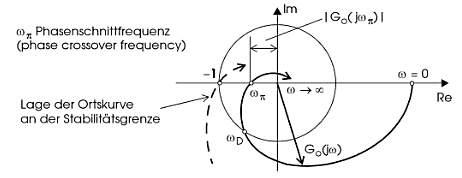
\includegraphics[width = .9\linewidth]{./images/Nyquistkurve}
	%% TODO: finish
	\iffalse
	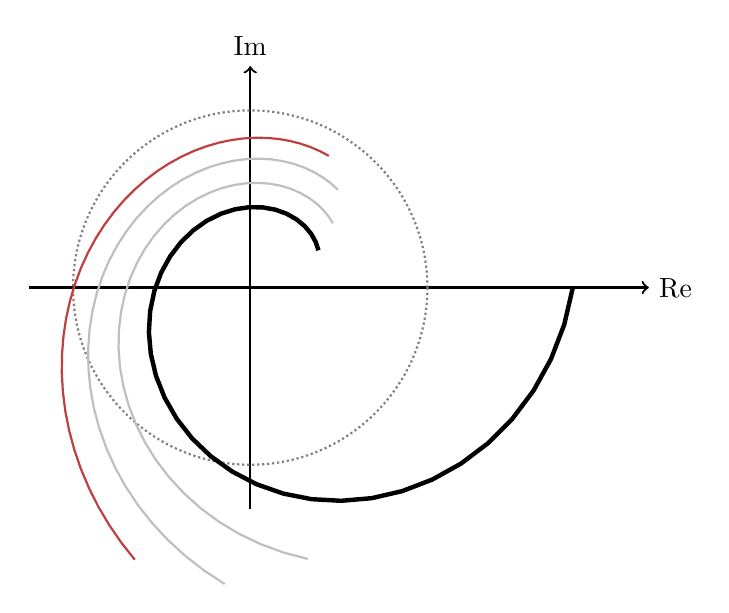
\begin{tikzpicture}
		\pgfmathsetmacro\radius{2.25}

		% axis and unit circle
		\draw[thick, ->] (-1.25*\radius, 0) to (2.25*\radius, 0) node[right] {Re};
		\draw[thick, ->] (0, -1.25*\radius) to (0, 1.25*\radius) node[above] {Im};
		\draw[gray, thick, densely dotted] (0,0) circle (\radius);

		% scaled curves (increase k)
		\foreach \scale / \color / \domain in {%
			1.3/lightgray/1.2:{1.5*pi},
			1.6/lightgray/1.4:{1.4*pi},
			1.86/red!50!gray/1.6:{1.3*pi}%
		}{
			\draw[draw = \color, thick, domain = \domain, samples = 40] plot
				({\scale * \radius * (1/4 + \x / 4 * cos(\x * 180/pi))},
				 {\scale * \radius * \x / 4 * sin(\x * 180/pi)});
		}

		% curve
		\draw[black, ultra thick, domain = 1:{2*pi}, samples = 40] plot
			({\radius * (1/4 + \x / 4 * cos(\x * 180/pi))}, {\radius * \x / 4 * sin(\x * 180/pi)});

	\end{tikzpicture}
	\fi
\end{figure}
Der geschlossene Regelkreis ist genau dann stabil, wenn beim Durchlauf der Ortskurve des offenen Regelkreises \(G_0\) in Richtung zunehmender Frequenz der kritische Punkt \(-1\) ``zur Linken'' liegt, daher nicht umschlungen wird.

Dies ist eine vereinfachte Form des Nyquist-Kriteriums und setzt einen stabilen offenen Kreis voraus (Prozess mit Ausgleich), der auch noch durch ein I-Glied ergänzt sein darf (Prozess ohne Ausgleich).

\subsection{Phasenreserve und Verstärkungsreserve \formelbuch{128-129}}

\begin{figure}[h!]
	\centering
	% 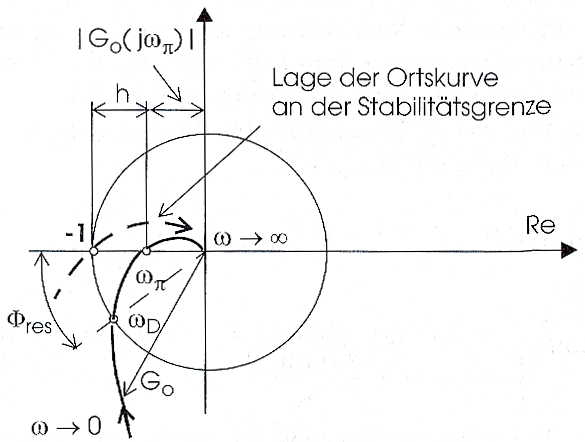
\includegraphics[width = .9\linewidth]{./images/phasenreserve.png}
	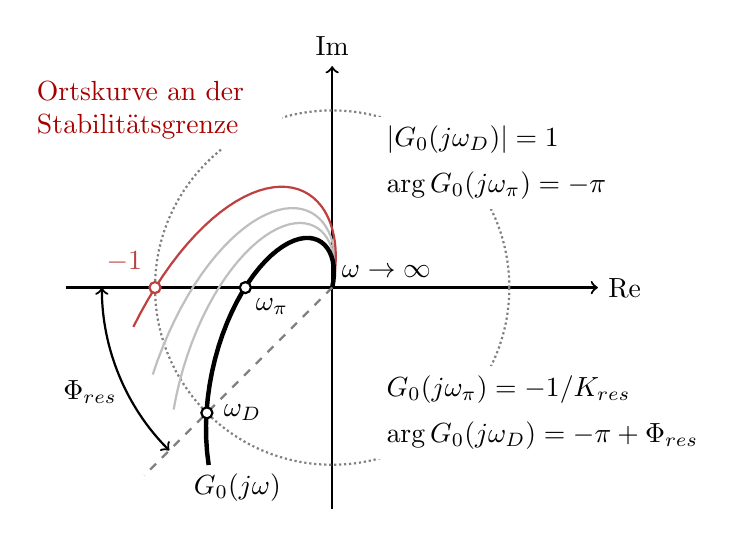
\begin{tikzpicture}
		\pgfmathsetmacro\radius{2.25}

		% axis and unit circle
		\draw[thick, ->] (-1.5*\radius, 0) to (1.5*\radius, 0) node[right] {Re};
		\draw[thick, ->] (0, -1.25*\radius) to (0, 1.25*\radius) node[above] {Im};
		\draw[gray, thick, densely dotted] (0,0) circle (\radius);

		% scaled curves (increase k)
		\foreach \scale / \color / \domain in {%
			1.3/lightgray/0:2.1,
			1.6/lightgray/0:1.9,
			2.03/red!50!gray/0:1.7%
		}{
			\draw[draw = \color, thick, domain = \domain, samples = 40] plot
				({\scale * \radius * -1 * \x / 3 * sin(\x * 180 / pi - 20)}, 
				 {\scale * \radius * \x / 2 * cos(\x * 180 / pi)});
		}

		% instability at -1
		\node[
			circle,
			draw = red!50!gray, thick, solid,
			fill = white,
			minimum size = 4pt,
			inner sep = 0pt,
			label = {[text = red!50!gray]120:\(-1\)},
		] at (-1*\radius,0) {};

		\node[
			red!65!black,
			fill = white,
			text width = 3cm,
		] at (-\radius, \radius) {%
			Ortskurve an der Stabilit\"atsgrenze%
			% \(K_{R\pi}G_0(j\omega_\pi) = -1\)
		};

		% curve
		\draw[black, ultra thick, domain = 0:2.5, samples = 40] plot
			({\radius * -1 * \x / 3 * sin(\x * 180 / pi - 20)},
			 {\radius * \x / 2 * cos(\x * 180 / pi)});

		\node[below right] at (230:1.3*\radius) {\(G_0(j\omega)\)};
		\node[above right] at (0,0) {\(\omega \to \infty\)};

		% phase reserve
		\draw[thick, dashed, gray] (0,0) to (225:1*\radius)
			node[
				circle,
				draw = black, thick, solid,
				fill = white,
				minimum size = 4pt,
				inner sep = 0pt,
				label = {[text = black]0:\(\omega_D\)},
			] {}
			to (225:1.5*\radius);

		\draw[thick, <->] (225:1.3*\radius) arc (225:180:1.3*\radius)
			node[left, pos = .4] {\(\Phi_\text{res}\)};

		% amplification reserve
		\node[
			circle,
			draw = black, thick, solid,
			fill = white,
			minimum size = 4pt,
			inner sep = 0pt,
			label = {[text = black, label distance = -2pt]-45:\(\omega_\pi\)},
		] at (-.49*\radius,0) {};

		% few more infos
		\matrix[
			anchor = west,
			nodes = {
				fill = white,
				text = black,
			},
		] at (.2*\radius, 0) {
			\node {\(|G_0(j\omega_D)| = 1\)}; \\
			\node {\(\arg G_0(j\omega_\pi) = - \pi\)}; \\[20mm]
			\node {\(G_0(j\omega_\pi) = -1/K_\text{res}\)}; \\
			\node {\(\arg G_0(j\omega_D) = -\pi + \Phi_\text{res}\)}; \\
		};

	\end{tikzpicture}
\end{figure}

% \subsubsection{Vorgehen beim Einstellen von P-Regler}
% \textbf{Gegeben \(\Phi_\text{res}\) finde \(K_\text{res}\)}
% \begin{enumerate}
% 	\item Mit \(\arg G_0(\omega_D) = -\pi + \Phi_\text{res}\) Durchtrittsfrequenz \(\omega_D\) bestimmen.
% 	\item Dann \(K_\text{res} \cdot |G_0(j\omega_D)| = 1\) nach \(K_\text{res}\) aufl\"osen.
% 	\item Das P-Glied muss mindestens \(K_R \leq 1 / K_\text{res}\) haben.
% \end{enumerate}
% 
% \textbf{Gegeben \(K_{\text{res}}\) finde  \(\Phi_\text{res}\)}
% \begin{enumerate}
% 	\item Mit \(1 = K_\text{res} \cdot |G_0(j\omega_\pi)|\) Phasenschnittfrequenz \(\omega_\pi\) bestimmen.
% 	\item 
% \end{enumerate}

\subsection{Stabilit\"at in Bodediagramme \formelbuch{140}}

\subsection{Alternative stabilit\"atskriterien \formelbuch{141}}

Eine \emph{notwendige} Stabilit\"atsbedingung f\"ur das charakteristische Polynom
\[
	a_n \lambda^n + \cdots + a_2 \lambda^2 + a_1 \lambda + a_0
\]
besteht darin, dass alle Koeffizienten \(a_n, \ldots, a_0\) dasselbe Vorzeichen haben.
Bei Systemen 1. und 2. Ordnung ist die Vorzeichenregel \emph{hinreichend} f\"ur die Stabilit\"at.

\subsection{Stabilitätssatz für die Sprungantwort}
Ein LTI-System ist genau dann stabil, wenn die Sprungantwort auf einen konstantem Wert zustrebt.
